	\section*{Exercice 2 (5 points)}
	

	\subsection*{1.}
	On peut dresser un arbre pondéré de probabilités :
	
	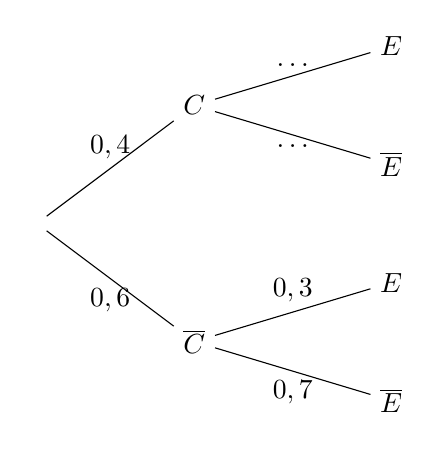
\begin{tikzpicture}
	[level 1/.style={level distance=2cm,
		sibling distance=3cm},
	level 2/.style={level distance=2.5cm,
		sibling distance=1.5cm}]
	\node {} [grow'=right]
	child {node {$C$}
		child {node {$E$}
			edge from parent node[above] {$\ldots$}
		}
		child {node {$\overline E$}
			edge from parent node[below] {$\ldots$}
		}
		edge from parent node[above] {$0,4$}
	}
	child {node {$\overline C$}
		child {node {$E$}
			edge from parent node[above] {$0,3$}
		}
		child {node {$\overline E$}
			edge from parent node[below] {$0,7$}
		}
		edge from parent node[below] {$0,6$}
	}
	;
\end{tikzpicture}


	
	
	\begin{itemize}
		\item On a  $P(C) = 0,40$; 
		\item L’énoncé donne  $P(C \cap E) = 0,24$; 
		\item  L’énoncé donne également $ P_{\overline{C}}(E)= 0,30$.
	\end{itemize}
	
	
	\subsection*{2.}
	On a $P(C \cap E) = P(C) \times P_{\overline{C}}(E) = 0,6 \times 0,7 = 0,42$.
	
	\subsection*{3.}
	On a $P(C) \times P_C(E)= 0,4 \times P_C(E)= 0,24$. On en déduit que $P_C(E) = \frac{0,24}{0,4} = \frac{6}{10} = 0,6$.
	
	D’après la loi des probabilités totales :
	\[
	P(E) = P(E \cap C) + P(E \cap \overline{C}) = 0,4 \times 0,6 + 0,6 \times 0,3 = 0,24 + 0,18 = 0,42.
	\]
	
	\subsection*{4.}
	On a $P(C \cap E) = 0,4 \times 0,6 = 0,24$ et $P(C) \times P(E) = 0,4 \times 0,42 = 0,168$.
	
	Comme $P(C \cap E) \neq P(C) \times P(E)$, on en déduit que les évènements $C$ et $E$ ne sont pas indépendants.
	
